% LaTeX Präsentationsvorlage (2013) der TU Graz, rev12, 2013/01/31
% !TeX encoding = UTF-8
\documentclass{beamer}
% \documentclass[aspectratio=169]{beamer}
% \usetheme{tugraz2013}
% \usetheme[notes]{tugraz2013}
\usepackage{../common/beamerthemetugraz2013}
\usepackage{color}
\usepackage{multicol}
\usepackage{bbding}
\usepackage{wasysym}
\usepackage{caption}
% \usepackage{minted}

\usepackage{listings}
\usepackage{xcolor}

\definecolor{codegreen}{rgb}{0,0.6,0}
\definecolor{codegray}{rgb}{0.5,0.5,0.5}
\definecolor{codepurple}{rgb}{0.58,0,0.82}
\definecolor{backcolour}{rgb}{0.95,0.95,0.92}
\lstdefinestyle{mystyle}{
    backgroundcolor=\color{backcolour},   
    commentstyle=\color{codegreen},
    keywordstyle=\color{magenta},
    numberstyle=\tiny\color{codegray},
    stringstyle=\color{codepurple},
    basicstyle=\ttfamily\footnotesize,
    breakatwhitespace=false,         
    breaklines=true,                 
    captionpos=b,                    
    keepspaces=true,                 
    numbers=left,                    
    numbersep=5pt,                  
    showspaces=false,                
    showstringspaces=false,
    showtabs=false,                  
    tabsize=2
}

\lstset{style=mystyle}

\usepackage{picture}
\usepackage{rotating}
\definecolor{darkred}{rgb}{0.85,0.16,0.0}
\definecolor{darkgreen}{rgb}{0.16,0.70,0.27}

\usepackage{xcolor}


\newcommand{\hrefu}[2]{\underline{\href{#1}{#2}}}
\newcommand{\hyperlinku}[2]{\underline{\hyperlink{#1}{#2}}}
\newcommand{\smallurl}[1]{%
  \begin{flushleft}
    \tiny\url{#1}
  \end{flushleft}
}
\newcommand{\smalltext}[1]{%
  \begin{flushleft}
    \tiny{#1}
  \end{flushleft}
}
\newcommand{\red}[1]{{\color{red} #1}}
\newcommand{\blue}[1]{{\color{blue} #1}}
\newcommand{\darkgreen}[1]{\textcolor{darkgreen}{#1}}
\newcommand{\darkred}[1]{\textcolor{darkred}{#1}}

\newcommand*{\vpointer}{\vcenter{\hbox{\scalebox{1.5}{\large\pointer}}}}

\newcommand{\be}[1]{\begin{equation} \label{#1}}
\newcommand{\ee}{\end{equation}}
\newcommand{\bea}[1]{\begin{eqnarray} \label{#1}}
\newcommand{\eea}{\end{eqnarray}}
\newcommand{\bean}{\begin{eqnarray*}}
\newcommand{\eean}{\end{eqnarray*}}

\newcommand{\non}{\nonumber\\}
\newcommand{\eq}[1]{(\ref{#1})}
\newcommand{\difp}[2]{\frac{\partial #1}{\partial #2}}
\newcommand{\br}{{\bf r}}
\newcommand{\bR}{{\bf R}}
\newcommand{\bA}{{\bf A}}
\newcommand{\bB}{{\bf B}}
\newcommand{\bE}{{\bf E}}
\newcommand{\bm}{{\bf m}}
%\renewcommand{\bm}{{\bf m}}
\newcommand{\bn}{{\bf n}}
\newcommand{\bN}{{\bf N}}
\newcommand{\bp}{{\bf p}}
\newcommand{\bP}{{\bf P}}
\newcommand{\bF}{{\bf F}}
\newcommand{\by}{{\bf y}}
\newcommand{\bz}{{\bf z}}
\newcommand{\bZ}{{\bf Z}}
\newcommand{\bV}{{\bf V}}
\newcommand{\bv}{{\bf v}}
\newcommand{\bu}{{\bf u}}
\newcommand{\bx}{{\bf x}}
\newcommand{\bX}{{\bf X}}
\newcommand{\bW}{{\bf W}}
\newcommand{\bJ}{{\bf J}}
\newcommand{\bj}{{\bf j}}
\newcommand{\bk}{{\bf k}}
\newcommand{\bTheta}{{\bf \Theta}}
\newcommand{\btheta}{{\boldsymbol\theta}}
\newcommand{\bOmega}{{\bf \Omega}}
\newcommand{\bomega}{{\boldsymbol\omega}}
\newcommand{\brho}{{\boldsymbol\rho}}
\newcommand{\rd}{{\rm d}}
\newcommand{\rJ}{{\rm J}}
\newcommand{\ph}{{\varphi}}
\newcommand{\te}{\theta}
\newcommand{\tht}{\vartheta}
\newcommand{\vpar}{v_\parallel}
\newcommand{\vparkb}{v_{\parallel k b}}
\newcommand{\vparkm}{v_{\parallel k m}}
\newcommand{\Jpar}{J_\parallel}
\newcommand{\ppar}{p_\parallel}
\newcommand{\Bpstar}{B_\parallel^*}
\newcommand{\intpi}{\int\limits_{0}^{2\pi}}
\newcommand{\summ}{\sum \limits_{m=-\infty}^\infty}
\newcommand{\tb}{\tau_b(\uv)}
\newcommand{\bh}{{\bf h}}
\newcommand{\cE}{{\cal E}}
\newcommand{\bsigma}{{\boldsymbol\sigma}}
\newcommand{\bS}{{\mathbf S}}
\newcommand{\bI}{{\mathbf I}}
\newcommand{\odtwo}[2]{\frac{\rd #1}{\rd #2}}
\newcommand{\pdone}[1]{\frac{\partial}{\partial #1}}
\newcommand{\pdtwo}[2]{\frac{\partial #1}{\partial #2}}
\newcommand{\ds}{\displaystyle} % commands


%% Titelblatt-Einstellungen
\title[]
{Python 08}
\author[E.~Wachmann]{\scriptsize Elias Wachmann
}
\date{2024} % \today für heutiges Datum verwenden
\institute[Institute of Theoretical and Computational Physics]
{
}
\instituteurl{www.tugraz.at}
% \institutelogo{kurz.pdf}
%~ \additionallogo{merged_logos}
\AtBeginSection[]{
  \begin{frame}
  \vfill
  \centering
  \begin{beamercolorbox}[sep=8pt,center,shadow=true,rounded=true]{title}
    \usebeamerfont{title}\insertsectionhead\par%
  \end{beamercolorbox}
  \vfill
  \end{frame}
}
\lstset{
    literate={Ö}{{\"O}}1
             {Ä}{{\"A}}1
             {Ü}{{\"U}}1
             {ß}{{\ss}}1
             {ü}{{\"u}}1
             {ä}{{\"a}}1
             {ö}{{\"o}}1
}

%%%%%%%%%%%%%%%%%%%%%%%%%%%%%%%%%%%%%%%%%%%%%%%%%%%%%%%%%%%%%%%%%%%%%%%%%%%%
\begin{document}
%%%%%%%%%%%%%%%%%%%%%%%%%%%%%%%%%%%%%%%%%%%%%%%%%%%%%%%%%%%%%%%%%%%%%%%%%%%%
\titleframe

%\begin{frame}
%  \frametitle{Outline}
%  \tableofcontents%[hideallsubsections] 
%  \note{
%  	Meine Präsentation ist wie folgt strukturiert \ldots
%  }
%\end{frame}

\section*{Content}

\begin{frame}
\frametitle{Content}
  \tableofcontents
\end{frame}

%%%%%%%%%%%%%%%%%%%%%%%%%%%%%%%%%%%%%%%%%%%%%%%%%%%%%%%%%%%%%%%%%%%%%%%%%%%%
\section{Lambda functions}
\begin{frame}
  \frametitle{Lambda functions}
  \hrefu{https://www.w3schools.com/python/python\_lambda.asp}{Lambda functions} are small anonymous functions. They can take any number of arguments, but can only have one expression. \\They are useful for short functions that are only used once.\\
  \lstinputlisting[language=python, firstline=3, lastline=5]{examples/lambda1.py}
\end{frame}
\begin{frame}
  \frametitle{Lambda functions inside other functions (closure)}
  Maybe you want to create functions at runtime. This can be done using lambda functions inside other functions.\\
  \lstinputlisting[language=python, firstline=4, lastline=9]{examples/lambda2.py}
\end{frame}
\begin{frame}
  \frametitle{Lambda functions inside other functions (closure)}
  Create multiple functions using lists and a closure.\\
  \lstinputlisting[language=python, firstline=10, lastline=15]{examples/lambda2.py}
\end{frame}
\begin{frame}
  \frametitle{Lambda functions inside other functions (closure)}
  Create multiple functions using lists and a closure.\\
  \begin{center}
    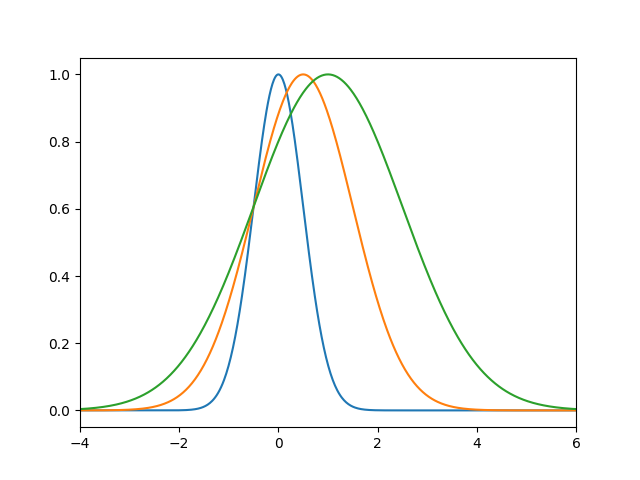
\includegraphics[width=0.65\textwidth]{examples/fig/lambda2.png}
  \end{center}
\end{frame}
\begin{frame}
  \frametitle{Lambda using multiple arguments}
  Lambda functions can take multiple arguments, just like normal functions.\\
  \lstinputlisting[language=python]{examples/lambda3.py}
  You can even specify default values for the arguments and nest lambda functions.
\end{frame}
\begin{frame}
  \frametitle{Lambda \& if / else}
  Compact way to find prime numbers.\\
  \lstinputlisting[language=python]{examples/lambda4.py}
  \textbf{Note:} The \texttt{<arg> if <condition> else <arg>} syntax is called a \hrefu{https://note.nkmk.me/en/python-if-conditional-expressions/}{conditional expression} which can also be used inside list/dict comprehensions and in returns.
\end{frame}
\section{Curve fitting}
\begin{frame}
  \frametitle{Curve fitting using \texttt{scipy}}
  With the \texttt{\hrefu{https://docs.scipy.org/doc/scipy/reference/generated/scipy.optimize.curve\_fit.html}{curve\_fit}} function from the \texttt{\hrefu{https://docs.scipy.org/doc/scipy/reference/index.html}{scipy}} module you can fit a function to data.\\
  % \vspace{5mm}
  \begin{center}
    \includegraphics[width=0.7\textwidth]{examples/fig/curve\_fit.png}
  \end{center}
\end{frame}
\begin{frame}
  \frametitle{Curve fitting using \texttt{scipy}}
  \lstinputlisting[language=python, firstline=3, lastline=13]{examples/curve_fit.py}
\end{frame}
\begin{frame}
  \frametitle{Curve fitting using \texttt{scipy}}
  \lstinputlisting[language=python, firstline=12]{examples/curve_fit.py}
\end{frame}
\begin{frame}
  \frametitle{Finding a minima using \texttt{scipy}}
  %fmin
  With the \texttt{\hrefu{https://docs.scipy.org/doc/scipy/reference/generated/scipy.optimize.fmin.html}{fmin}} function you can find the minima of a function.\\
  \begin{center}
    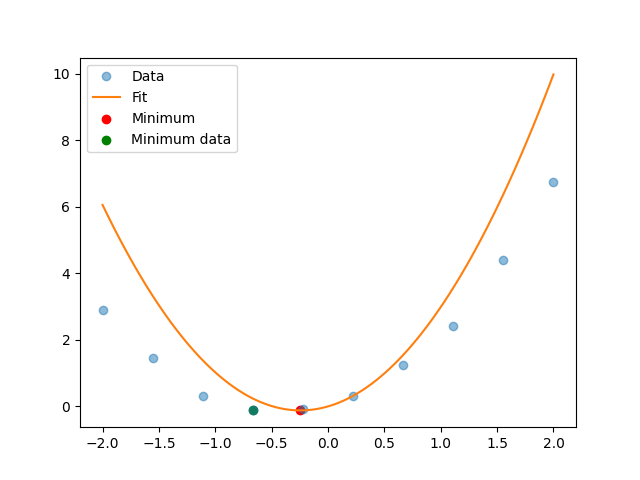
\includegraphics[width=0.7\textwidth]{examples/fig/fmin.png}
  \end{center}
\end{frame}
\begin{frame}
  \frametitle{Finding a minima using \texttt{scipy}}
  \lstinputlisting[language=python, firstline=3, lastline=12]{examples/fmin.py}
\end{frame}
\begin{frame}
  \frametitle{Finding a minima using \texttt{scipy}}
  \lstinputlisting[language=python, firstline=15, lastline=21]{examples/fmin.py}
\end{frame}
\begin{frame}
  \frametitle{Finding a minima using \texttt{scipy}}
  \lstinputlisting[language=python, firstline=22]{examples/fmin.py}
\end{frame}
\section{Interpolation}
\begin{frame}
  \frametitle{Difference between interpolation and curve fitting}
  Interpolation constructs new data points within the range of a discrete set of known data points.\\
  \vspace{5mm}
  Curve fitting is the process of constructing a curve, or mathematical function, that has the best fit to a series of data points.\\
  \vspace{5mm}
  While interpolation requires the function to \textbf{go through the data points}, curve fitting does not.\\
\end{frame}
\begin{frame}
  \frametitle{Interpolation using \texttt{scipy}}
  Scipy has a suite of functions for interpolation.\\
  \begin{center}
    \includegraphics[width=\textwidth]{examples/fig/top\_row\_interpolation.png}
  \end{center}
\end{frame}
\begin{frame}
  \frametitle{Interpolation using \texttt{scipy}}
  Scipy has a suite of functions for interpolation.\\
  \begin{center}
    \includegraphics[width=\textwidth]{examples/fig/bottom\_row\_interpolation.png}
  \end{center}
\end{frame}
\begin{frame}
  \frametitle{Interpolation using \texttt{scipy}}
  Using the \texttt{\hrefu{https://docs.scipy.org/doc/scipy/reference/generated/scipy.interpolate.interp1d.html}{interp1d}} function you can interpolate data.\\
  \begin{itemize}
    \item Nearest-neighbor interpolation ('nearest')
    \item Linear interpolation ('linear')
    \item Piecewise polynomial interpolation (PchipInterpolator)
    \item Cubic spline interpolation ('cubic')
  \end{itemize}
  For piecewise polynomial interpolation use \texttt{\hrefu{https://docs.scipy.org/doc/scipy/reference/generated/scipy.interpolate.PchipInterpolator.html}{PchipInterpolator}}.\\
\end{frame}
\begin{frame}
  \frametitle{Interpolation using \texttt{scipy}}
  \lstinputlisting[language=python, firstline=3, lastline=10]{examples/interpolate\_scipy.py}
\end{frame}
\begin{frame}
  \frametitle{Interpolation using \texttt{scipy}}
  \lstinputlisting[language=python, firstline=11, lastline=20]{examples/interpolate\_scipy.py}
\end{frame}

\section{Input / Output (I/O) [BONUS]}
\begin{frame}
  \frametitle{Input / Output (I/O)}
  We have considered the \texttt{\hrefu{https://docs.python.org/3/library/functions.html\#print}{print}} function to output text to the console.\\
  \vspace{5mm}
  \textbf{Input} can be read from the console using the \texttt{\hrefu{https://docs.python.org/3/library/functions.html\#input}{input}} function.\\
  \vspace{5mm}
  Users can also input arguments when calling a script from the command line. These arguments are stored in the \texttt{\hrefu{https://www.geeksforgeeks.org/how-to-use-sys-argv-in-python/}{sys.argv}} list.\\
\end{frame}
\begin{frame}
  \frametitle{Input -- \texttt{sys.argv}}
  Let's assume we have a script with the following content:\\
  \lstinputlisting[language=python]{examples/argv.py}
  We can now call this script from the command line and pass the number of iterations as an argument. 
\end{frame}
\begin{frame}
  \frametitle{Input -- \texttt{sys.argv}}
  We can now call this script from the command line and pass the number of iterations as an argument. 
  \begin{center}
    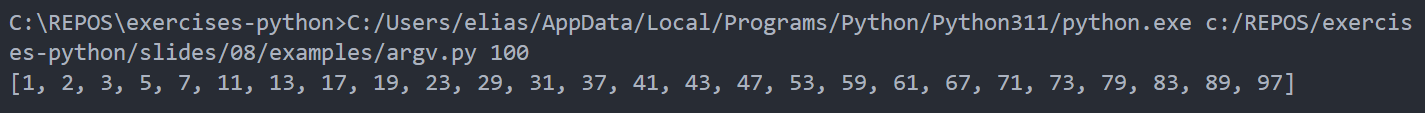
\includegraphics[width=\textwidth]{examples/fig/primes.png}
  \end{center}
  Entering 100 as an argument will return and print all prime numbers up to 100.
\end{frame}

\begin{frame}
  \frametitle{Input -- \texttt{input}}
  The \texttt{\hrefu{https://docs.python.org/3/library/functions.html\#input}{input}} function can be used to read user input from the console.\\
  \lstinputlisting[language=python]{examples/input1.py}
  \begin{center}
    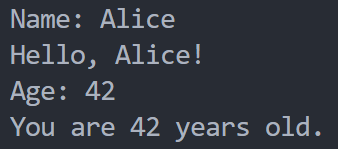
\includegraphics[width=0.35\textwidth]{examples/fig/input.png}
  \end{center}
\end{frame}

\begin{frame}
  \frametitle{Input -- check it before you wreck it!}
  User input is always read as a string and can be used as it or converted to other types.\\
  \begin{center}
    \textbf{Never trust user input!}
  \end{center} 
  Always check if the input is valid and convert it to the desired type. Otherwise, it might lead to unexpected behaviour, error or even security issues in the worst case.\\
\end{frame}
\begin{frame}
  \frametitle{Input -- check it before you wreck it!}
  Not checking input leads to unexpected behavior: 
  \begin{center}
    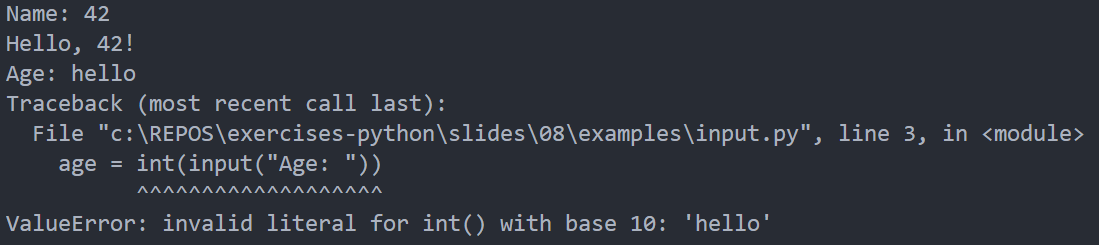
\includegraphics[width=\textwidth]{examples/fig/wronginput.png}
  \end{center}
  We can fix this by converting to the desired type in a try-except block.\\
\end{frame}

\begin{frame}
  \frametitle{Input -- check it before you wreck it!}
  We can fix this by converting to the desired type in a try-except block.\\
  \lstinputlisting[language=python]{examples/input2.py}
\end{frame}
\begin{frame}
  \frametitle{Input -- check it before you wreck it!}
  We can fix this by converting to the desired type in a try-except block. \\
  \vspace{5mm}
  This way the user gets useful feedback and the program does not crash.\\  
  \begin{center}
    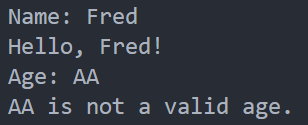
\includegraphics[width=0.35\textwidth]{examples/fig/inputchecked.png}
  \end{center}
\end{frame}
\begin{frame}
  \frametitle{Input -- check it before you wreck it!}
  Some code may be malicious and try to exploit your program.\\
  \lstinputlisting[language=python, firstline=4]{examples/memeater.py}
  If you input a large enough number the program will consume a lot of your RAM and the system may slow down or crash.\\
\end{frame}
\begin{frame}
  \frametitle{Input -- check it before you wreck it!}
  Python has some check which prevent this from happening $\rightarrow$ \texttt{MemoryError}.\\
  \begin{center}
    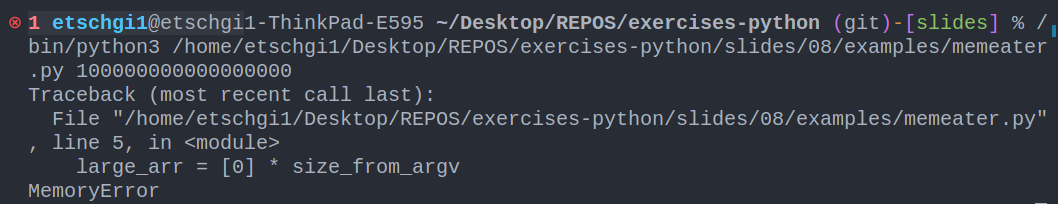
\includegraphics[width=\textwidth]{examples/fig/memerror.png}
  \end{center}
  But it is still good practice to check user input and prevent this from happening.\\
\end{frame}
\begin{frame}
  \frametitle{Input -- eval}
  The \texttt{\hrefu{https://docs.python.org/3/library/functions.html\#eval}{eval}} function can be used to evaluate a string as a Python expression.\\
  \lstinputlisting[language=python, firstline=3]{examples/eval.py}
  As you should know by now, this is dangerous and you shouldn't evaluate user input!\\
  Sometimes it may be useful though to dynamically evaluate equations (just like with closures).\\
\end{frame}
\begin{frame}
  \frametitle{Output -- a closer look at \texttt{print}}
  The \texttt{\hrefu{https://docs.python.org/3/library/functions.html\#print}{print}} function has a lot of options.\\
  \lstinputlisting[language=python, firstline=3]{examples/print.py}
  The \texttt{sep} argument can be used to specify the separator between the arguments and the \texttt{end} argument can be used to specify the end of the line.
  \texttt{\textbackslash n} \dots newline, \texttt{\textbackslash t} \dots tabulator, \texttt{\textbackslash r} \dots carriage return.
\end{frame}
\begin{frame}
  \frametitle{Output -- a closer look at colors}
  How to print colored text to the console?\\
  Use \hrefu{https://en.wikipedia.org/wiki/ANSI\_escape\_code}{escape sequences}!\\
  \lstinputlisting[language=python, firstline=3]{examples/color.py}
\end{frame}
\begin{frame}
  \frametitle{Output -- a closer look at colors}
  Output in the console:\\
  \begin{center}
    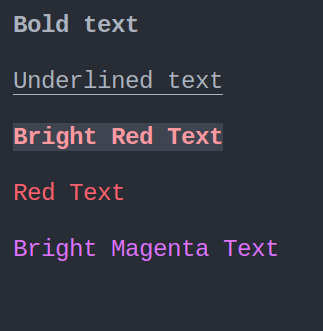
\includegraphics[width=0.45\textwidth]{examples/fig/colors.png}
  \end{center}
\end{frame}
% \section{File I/O}
% \begin{frame}
%   \frametitle{File I/O -- Basics}
%   Python uses \hrefu{https://docs.python.org/3/reference/compound_stmts.html\#with}{with} statements to open and close files.\\
%   \lstinputlisting[language=python]{examples/fileio1.py}
% \end{frame}
% \begin{frame}
%   \frametitle{File I/O -- file modes}
%   The \texttt{open} function can be used to open files in different modes (multiple are possible):\\
%   \begin{table}[h]
%   \centering
%   \begin{tabular}{|c|c|}
%   \hline
%   \textbf{File Mode} & \textbf{Description} \\ \hline
%   \texttt{r} & Read mode \\ \hline
%   \texttt{w} & Write mode \\ \hline
%   \texttt{x} & Exclusive creation mode \\ \hline
%   \texttt{a} & Append mode \\ \hline
%   \texttt{b} & Binary mode \\ \hline
%   \texttt{t} & Text mode \\ \hline
%   \texttt{+} & Read and write mode \\ \hline
%   \end{tabular}
%   \label{tab:file-modes}
%   \end{table}
% \end{frame}

% \begin{frame} \frametitle{File I/O -- Reading Files} To read the contents of a file, you can use the \texttt{\hrefu{https://docs.python.org/3/tutorial/inputoutput.html\#methods-of-file-objects}{read()}} method of the file object. This method reads the entire contents of the file and returns it as a string.

%   \lstinputlisting[language=python]{examples/fileio2.py}
  
%   In this example, we open the file \texttt{input.txt} in read mode (\texttt{r}), read its contents using the \texttt{\hrefu{https://docs.python.org/3/tutorial/inputoutput.html\#methods-of-file-objects}{read()}}  method, and print the contents to the console. \end{frame}
  
%   \begin{frame} \frametitle{File I/O -- Writing Files} To write to a file, you can use the \texttt{\hrefu{https://docs.python.org/3/tutorial/inputoutput.html\#methods-of-file-objects}{write()}} method of the file object. This method writes the specified string to the file.
  
%   \lstinputlisting[language=python, lastline=3]{examples/fileio3.py}
  
%   In this example, we open the file \texttt{example.txt} in write mode (\texttt{w}), write some strings to the file using the \texttt{\hrefu{https://docs.python.org/3/tutorial/inputoutput.html\#methods-of-file-objects}{write()}} method. 
% \end{frame}
% \begin{frame}
%   \frametitle{File I/O -- Reading multiple lines}
%   To read multiple lines from a file, you can use the \texttt{\hrefu{https://docs.python.org/3/tutorial/inputoutput.html\#methods-of-file-objects}{readlines()}} method of the file object. This method reads the entire contents of the file, and returns each line as an item in a list.
%   \lstinputlisting[language=python, firstline=4]{examples/fileio3.py}
%   You do not need to close the file when using the \texttt{with} statement. It is automatically closed when the \texttt{with} block is exited.
% \end{frame}

% \begin{frame}
%   \frametitle{File I/O -- Binary files}
%   To read or write binary files, you can use the \texttt{\hrefu{https://docs.python.org/3/tutorial/inputoutput.html\#methods-of-file-objects}{rb}} and \texttt{\hrefu{https://docs.python.org/3/tutorial/inputoutput.html\#methods-of-file-objects}{wb}} modes, respectively:
%   \lstinputlisting[language=python, firstline=3]{examples/fileio4.py}
%   But how do I know what is in there \dots ?
% \end{frame}
% \begin{frame}
%   \frametitle{File I/O -- Encoding}
%   There are many \hrefu{https://en.wikipedia.org/wiki/Character_encoding}{encodings} for text files.\\
%   \begin{itemize}
%     \item ASCII: 7-bit encoding, 128 characters
%     \item Unicode: 16-bit encoding, 65536 characters
%     \item UTF-8: 8-bit encoding, variable length, ASCII compatible
%     \item ISO-8859-1: 8-bit encoding, 256 characters (Latin-1)
%   \end{itemize}
%   To interpret a file in the right way, you have to specify the encoding.\\
% \end{frame}
% \begin{frame}
%   \frametitle{File I/O -- Encoding}
%   Specify the encoding when opening the file using the \texttt{encoding} argument:
%   \lstinputlisting[language=python]{examples/fileio5.py}
%   This will fail! Why? 
% \end{frame}
% \begin{frame}
%   \frametitle{File I/O -- Encoding}
%   The specified encoding has to match the encoding of the file!\\
%   \vspace{5mm}
%   The file was written using \texttt{UTF-8} encoding and later read using \texttt{ASCII} encoding which is doomed to fail, since an \glq Ö\grq is in the textfile.\\
%   \begin{center}
%     \includegraphics[width=\textwidth]{examples/fig/ascii\_fail.png}
%   \end{center}
% \end{frame}
% \section{ASCII Encoding}
% \begin{frame}
%   \frametitle{ASCII - Table}
%     \hrefu{https://de.wikipedia.org/wiki/American_Standard_Code_for_Information_Interchange}{ASCII} (American Standard Code for Information Interchange) is a character encoding standard that assigns unique numeric codes to each character in the English alphabet, as well as various punctuation marks and other symbols.
% \end{frame}
% \begin{frame}
%   \frametitle{ASCII - Table}
%   \begin{center}
%     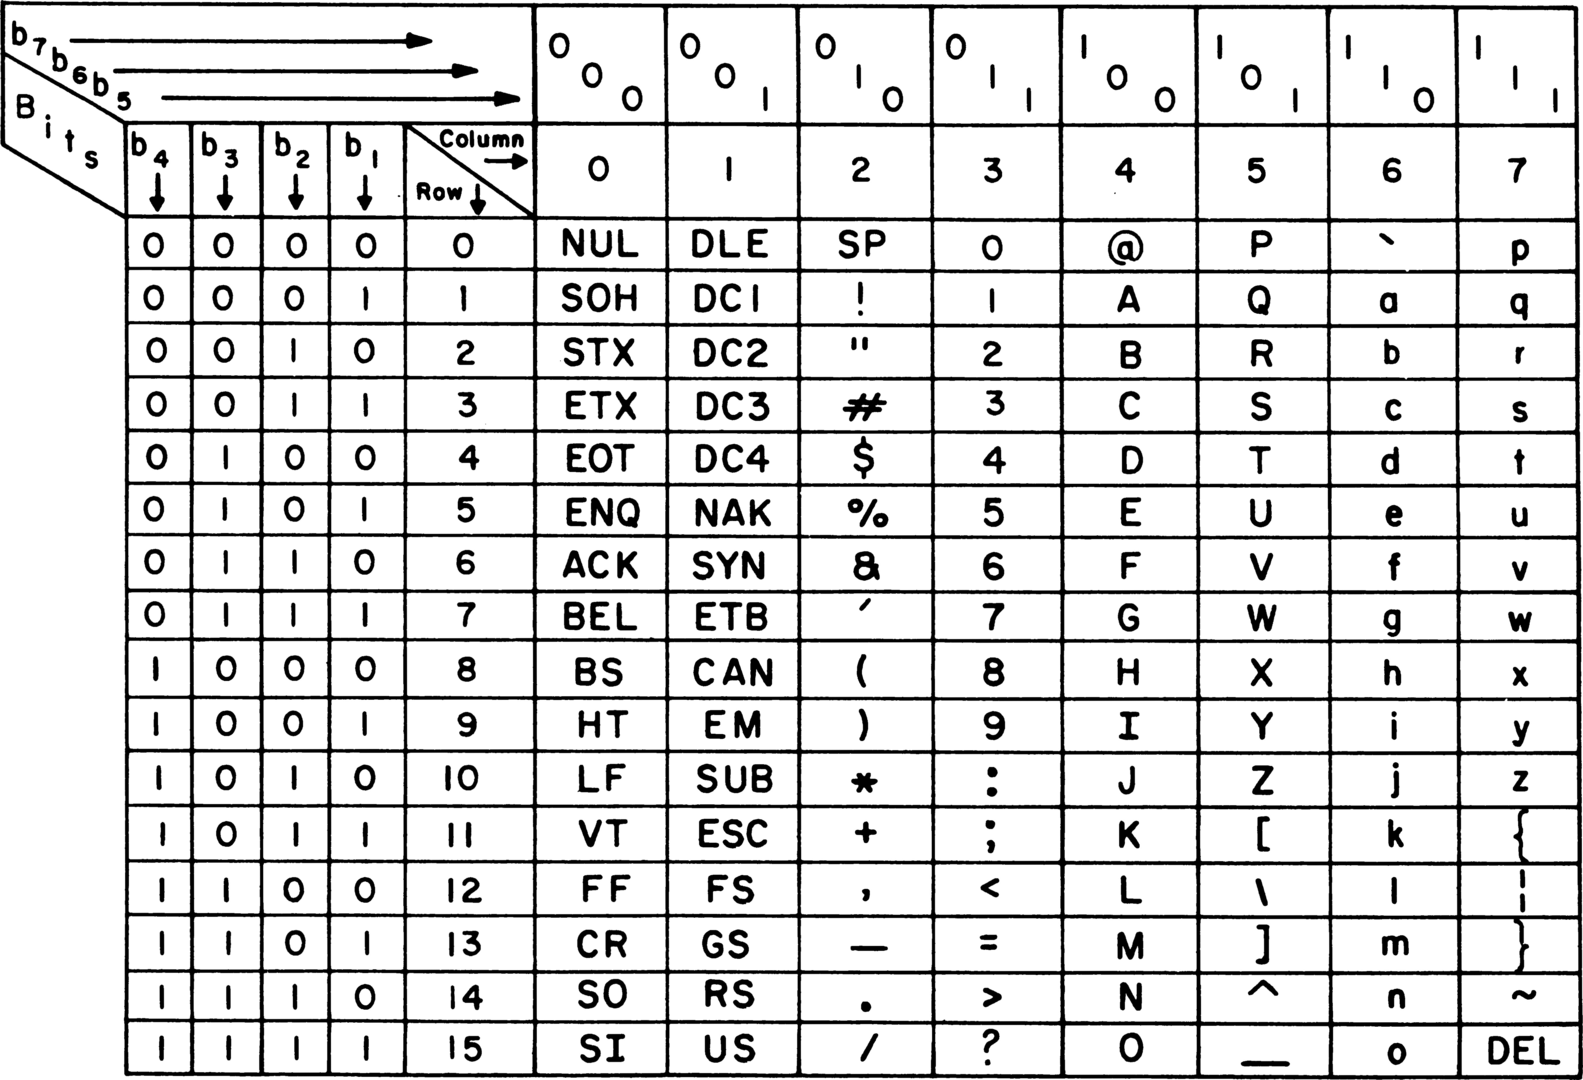
\includegraphics[width=0.75\textwidth]{examples/fig/ASCII.png}
%   \end{center}
%   \begin{flushleft}
%     \vspace{-4mm}
%     \tiny\url{https://de.wikipedia.org/wiki/American\_Standard\_Code\_for\_Information\_Interchange\#/media/Datei:USASCII\_code\_chart.png}
%   \end{flushleft}
% \end{frame}
% \begin{frame}
%   \frametitle{ASCII - Table}
%   This way everything is up to interpretation: 
%   You can read the file as ASCII if there are no special characters in it.:
%   \lstinputlisting[language=python, lastline=5]{examples/ascii.py}
% \end{frame}
% \begin{frame}
%   \frametitle{Using other encodings}
%   With another encoding you can read special characters such as \glq Ö\grq:
%   \lstinputlisting[language=python, firstline=6]{examples/ascii.py}
% \end{frame}
% \section{pickle}
% \begin{frame}
%   \frametitle{pickle}
%   \texttt{\hrefu{https://docs.python.org/3/library/pickle.html}{pickle}} is a module that allows you to store almost any Python object (lists, dictionaries, \dots) in a file.\\
%   \vspace{5mm}
%   \texttt{\hrefu{https://docs.python.org/3/library/pickle.html}{pickle}} is a binary format, so you have to open the file in binary mode (\texttt{wb} or \texttt{rb}).\\
%   \vspace{5mm}
%   Use the \texttt{\hrefu{https://docs.python.org/3/library/pickle.html\#pickle.dump}{dump()}} method to write an object to a file, and the \texttt{\hrefu{https://docs.python.org/3/library/pickle.html\#pickle.load}{load()}} method to read an object from a file.
% \end{frame}
% \begin{frame}
%   \frametitle{pickle -- Example}
%   \lstinputlisting[language=python]{examples/pickle\_example.py}
% \end{frame}
% \section{csv-Import (built-in)}
\begin{frame}
  \frametitle{Import csv-files}
  \texttt{\hrefu{https://docs.python.org/3/library/csv.html}{csv}} is a module that allows you to read and write csv-files.\\
  \vspace{5mm}
  \texttt{\hrefu{https://docs.python.org/3/library/csv.html}{csv}} is a text format, so you have to open the file in text mode (\texttt{w} or \texttt{r}).\\
  \vspace{5mm}
  To read a file use the \texttt{\hrefu{https://docs.python.org/3/library/csv.html\#csv.reader}{reader()}} method, to write a file use the \texttt{\hrefu{https://docs.python.org/3/library/csv.html\#csv.writer}{writer()}} method.
\end{frame}
\begin{frame}
  \frametitle{Import csv-files -- Example (csv)}
  \lstinputlisting[language=python]{examples/csv\_basic.py}
\end{frame}
\begin{frame}
  \frametitle{Import csv-files -- Example (csv)}
  Wow, that was a lot of code!\\
  Isn't there a better way?\\
  \vspace{5mm}
  Maybe do everything in one line?\\
  \vspace{5mm}
  Use \hrefu{https://pandas.pydata.org/pandas-docs/stable/}{pandas} inbuilt \hrefu{https://pandas.pydata.org/pandas-docs/stable/reference/api/pandas.read\_csv.html}{csv-import function} instead:
  \lstinputlisting[language=python]{examples/csv\_pandas.py}
\end{frame}
%%%%%%%%%%%%%%%%%%%%%%%%%%%%%%%%%%%%%%%%%%%%%%%%%%%%%%%%%%%%%%%%%%%%%%%%%%%%

\end{document}
%%%%%%%%%%%%%%%%%%%%%%%%%%%%%%%%%%%%%%%%%%%%%%%%%%%%%%%%%%%%%%%%%%%%%%%%%%%%

%% EOF
